\subsection{Database}

Dimulai dengan membuat sebuah database menggunakan MYSQL. Dengan adanya XAMPP akan mempermudah kita dalam membuat sebuah web yang sudah dilengkapi dengan Apache, MySQL dan PhP. Oleh karna itu, kita diharuskan menginstal terlebih dahulu XAMPPnya lalu jalankan Apache dan MySQLnya dengan mengklik tombol button start.

\begin{figure}[H]
	\centering
	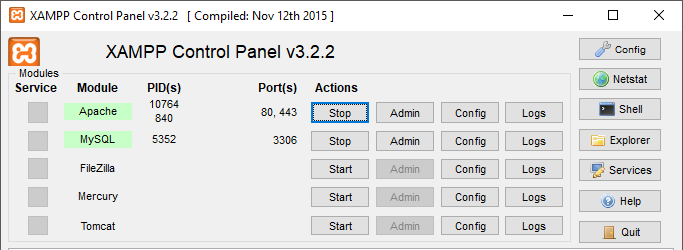
\includegraphics[width=7cm]{figures/database/1.png}
\end{figure}

\noindent
Seperti yang dapat kita lihat Apache dan MySQLnya sudah dijalankan, sehingga kita dapat memulai membuat database . Kemudian jalankan url http://localhost/phpmyadmin/ pada browser.

\begin{figure}[H]
\centering
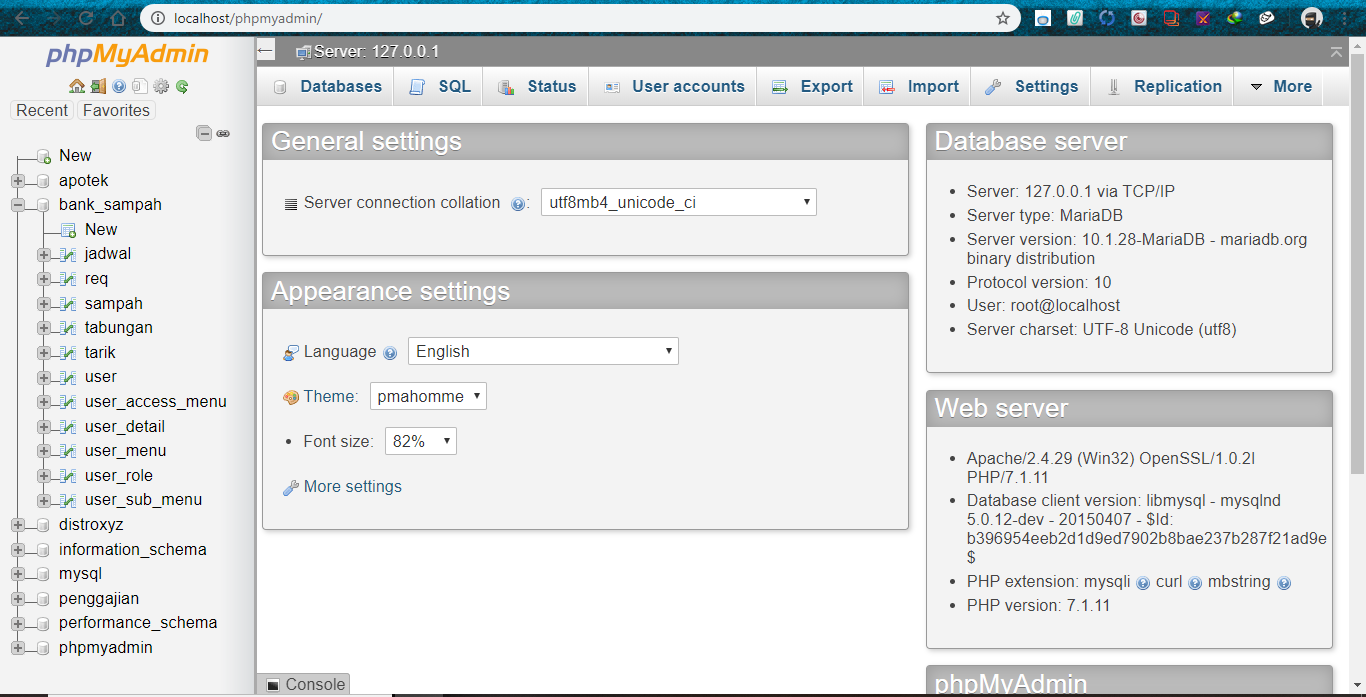
\includegraphics[width=1\textwidth]{figures/database/2.png}
\end{figure}

\noindent
Pada gambar di atas merupakan tampilan awal ketika kita membuka url http://localhost/phpmyadmin/, ketika url tersebut berhasil kita buka maka selanjutnya yaitu kita membuat database dengan nama bank\_sampah. Dimulai dengan mengklik menu SQL, lalu ketikan script ini “ CREATE DATABASE 'bank\_sampah' “ kemudian klik Go untuk mengekseskusinya.

\begin{figure}[H]
\centering
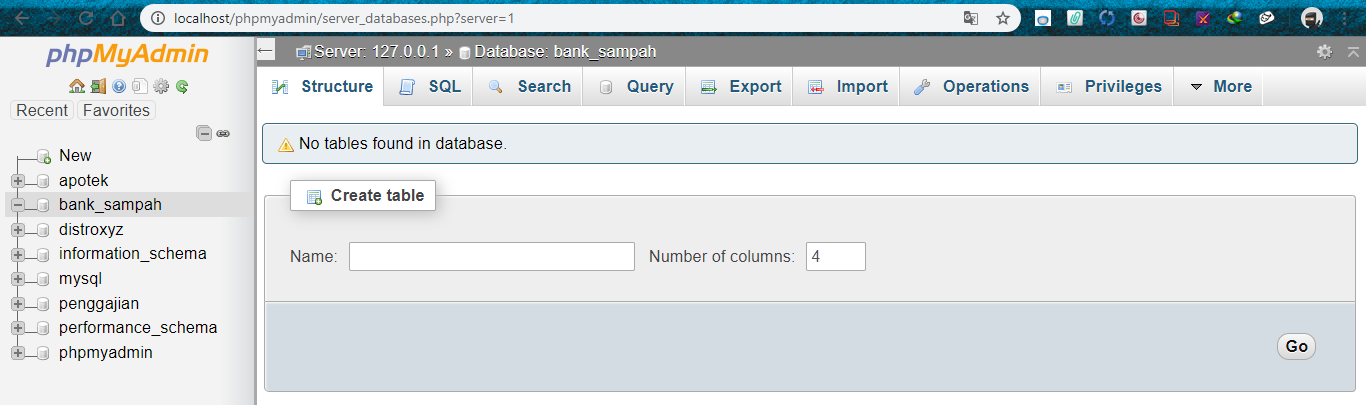
\includegraphics[width=1\textwidth]{figures/database/3.png}
\end{figure}

\noindent
Kita berhasil membuat data baru, dilanjut dengan membuat tabel-tabel untuk menyimpan data-data yang akan dibutuhkan pada aplikasi kita. Caranya klik menu SQL. Pertama kita akan membuat table jadwal. Ketikan script berikut dan untuk mengeksekusinya klik Go.

\lstinputlisting[firstline=31, lastline=35, language=SQL]{src/bank-sampah/bank_sampah.sql}

\begin{figure}[H]
\centering
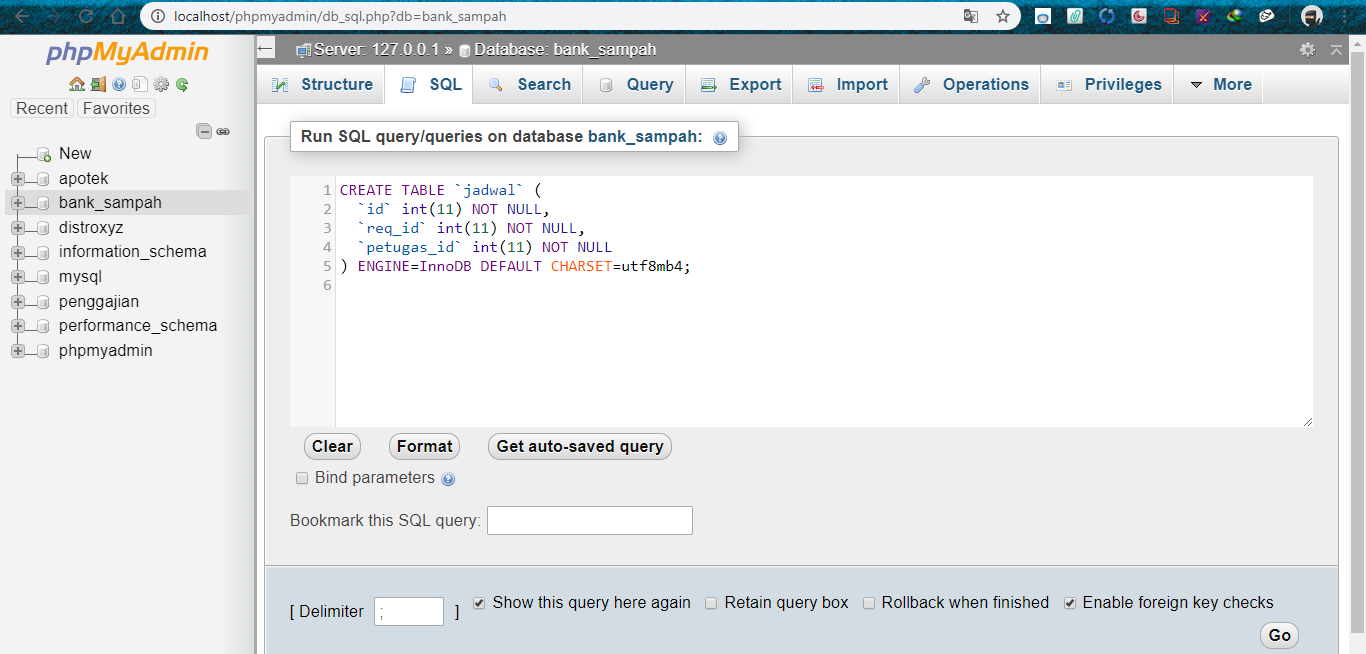
\includegraphics[width=1\textwidth]{figures/database/4.png}
\end{figure}

\noindent
Dilanjut dengan membuat tabel req. Caranya masih sama dengan sebelumnya, ketikan script berikut dan untuk mengekseskusinya klik Go.

\lstinputlisting[firstline=60, lastline=66, language=SQL]{src/bank-sampah/bank_sampah.sql}

\begin{figure}[H]
\centering
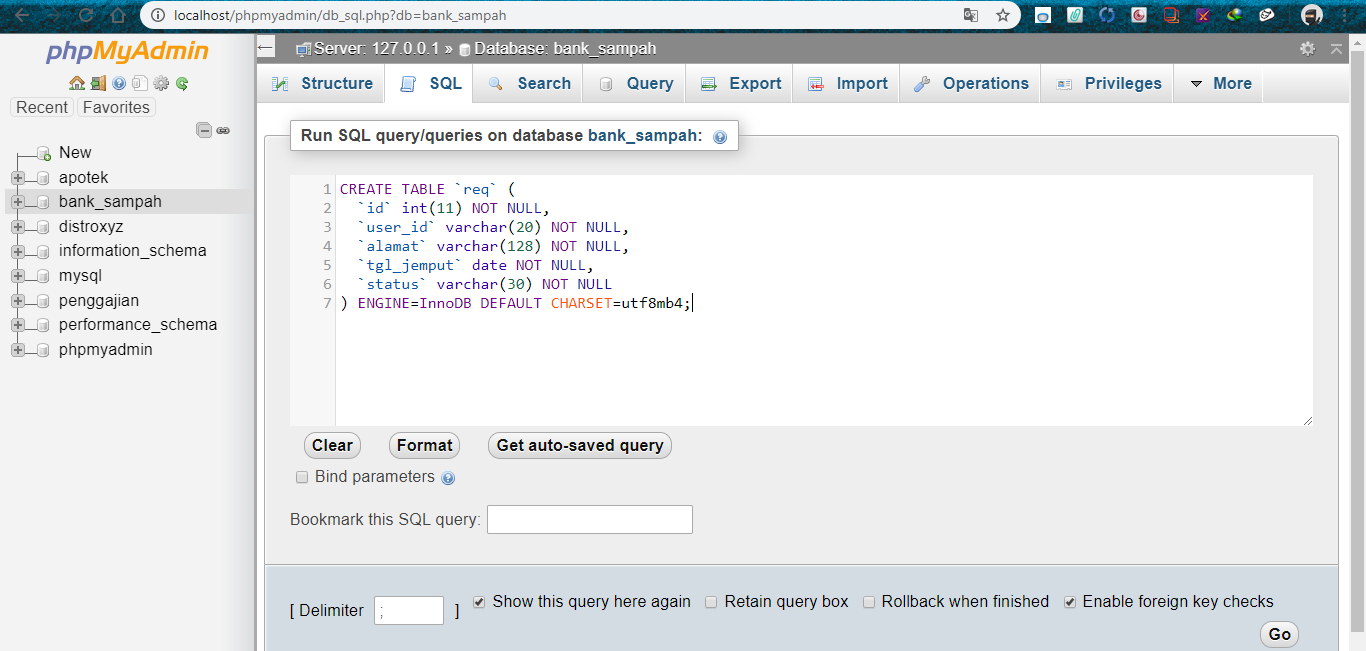
\includegraphics[width=1\textwidth]{figures/database/5.png}
\end{figure}

\noindent
Dilanjut dengan membuat tabel sampah. Caranya masih sama dengan sebelumnya, ketikan script berikut dan untuk mengekseskusinya klik Go.

\lstinputlisting[firstline=92, lastline=96, language=SQL]{src/bank-sampah/bank_sampah.sql}

\begin{figure}[H]
\centering
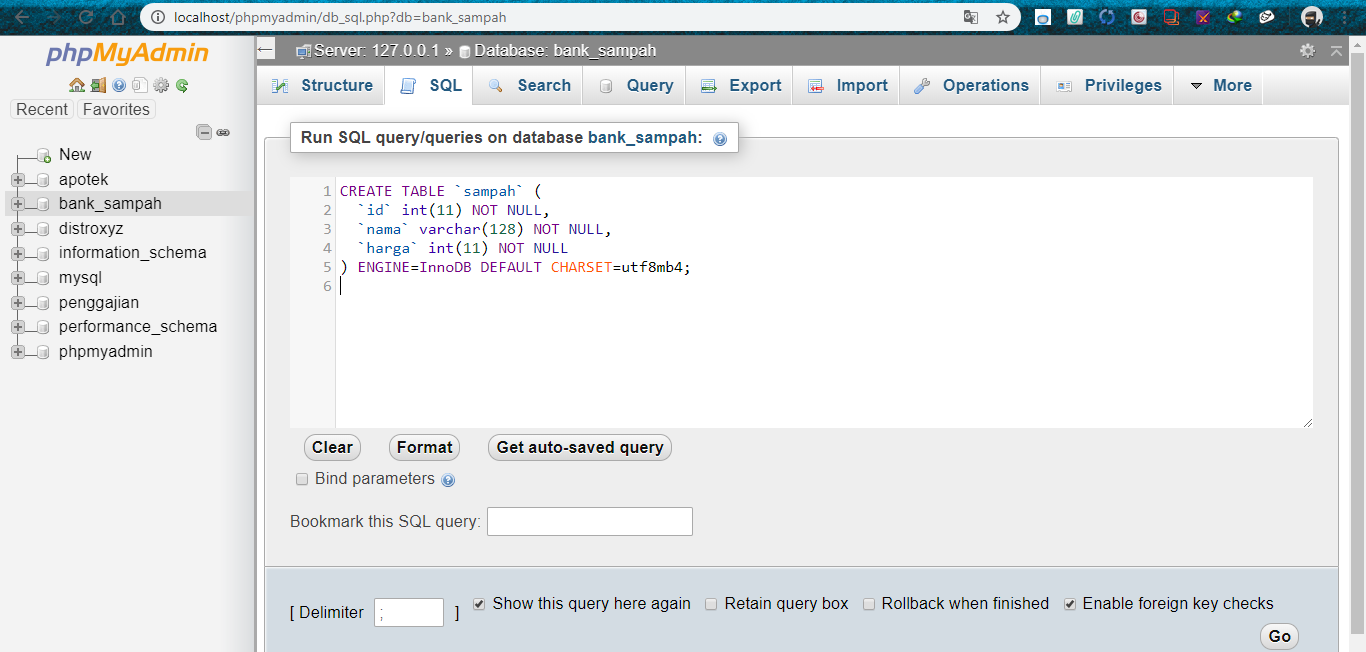
\includegraphics[width=1\textwidth]{figures/database/6.png}
\end{figure}

\noindent
Dilanjut dengan membuat tabel tabungan. Caranya masih sama dengan sebelumnya, ketikan script berikut dan untuk mengekseskusinya klik Go.

\lstinputlisting[firstline=120, lastline=126, language=SQL]{src/bank-sampah/bank_sampah.sql}

\begin{figure}[H]
\centering
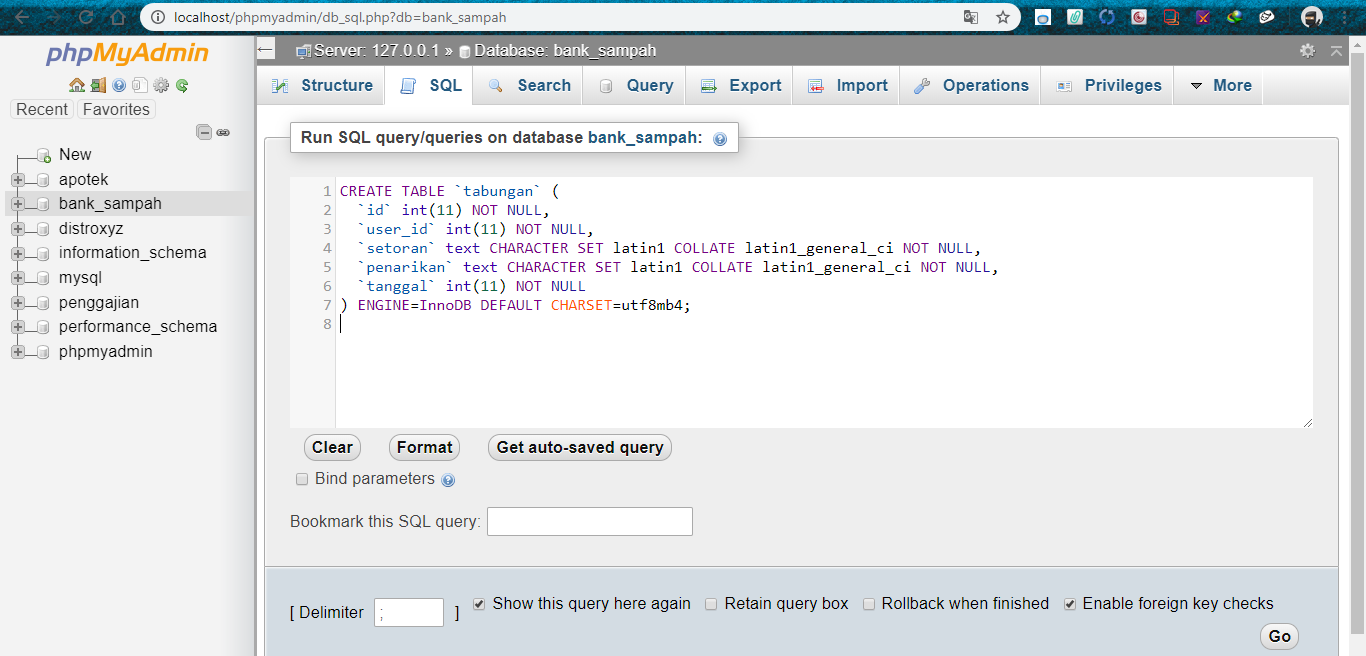
\includegraphics[width=1\textwidth]{figures/database/7.png}
\end{figure}

\noindent
Dilanjut dengan membuat tabel tarik. Caranya masih sama dengan sebelumnya, ketikan script berikut dan untuk mengekseskusinya klik Go.

\lstinputlisting[firstline=156, lastline=162, language=SQL]{src/bank-sampah/bank_sampah.sql}

\begin{figure}[H]
\centering
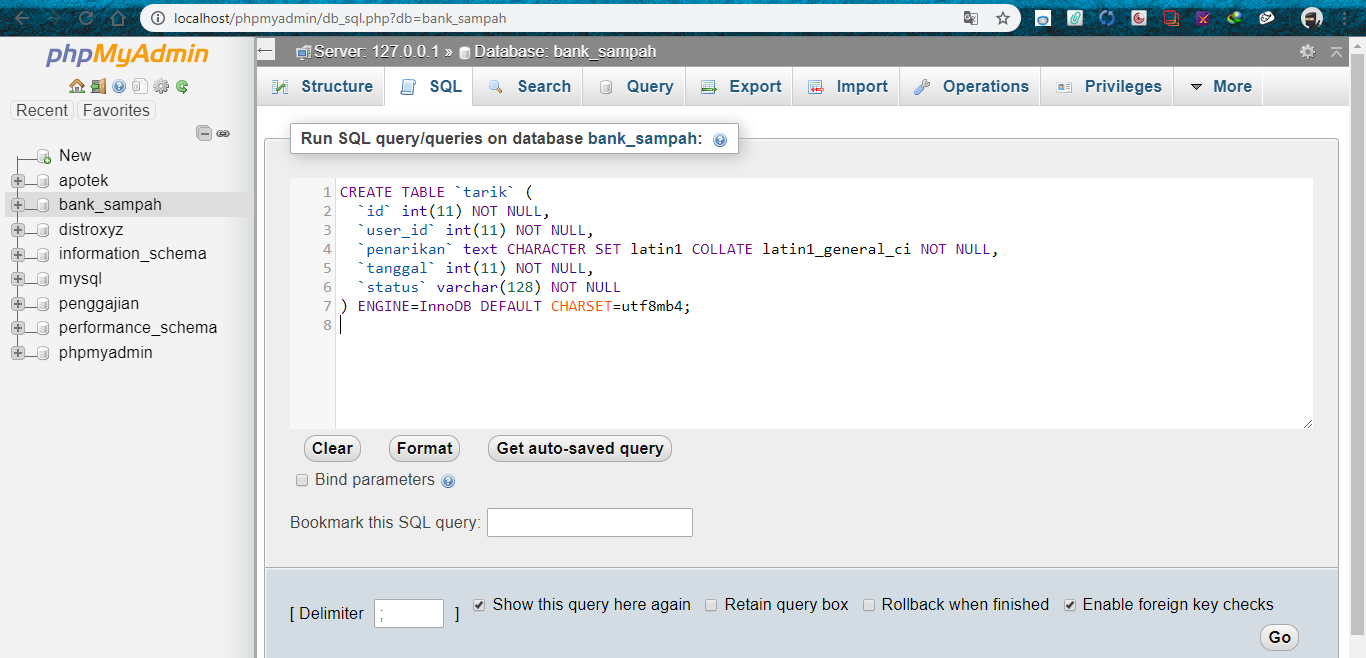
\includegraphics[width=1\textwidth]{figures/database/8.png}
\end{figure}

\noindent
Dilanjut dengan membuat tabel user. Caranya masih sama dengan sebelumnya, ketikan script berikut dan untuk mengekseskusinya klik Go.

\lstinputlisting[firstline=181, lastline=190, language=SQL]{src/bank-sampah/bank_sampah.sql}

\begin{figure}[H]
\centering
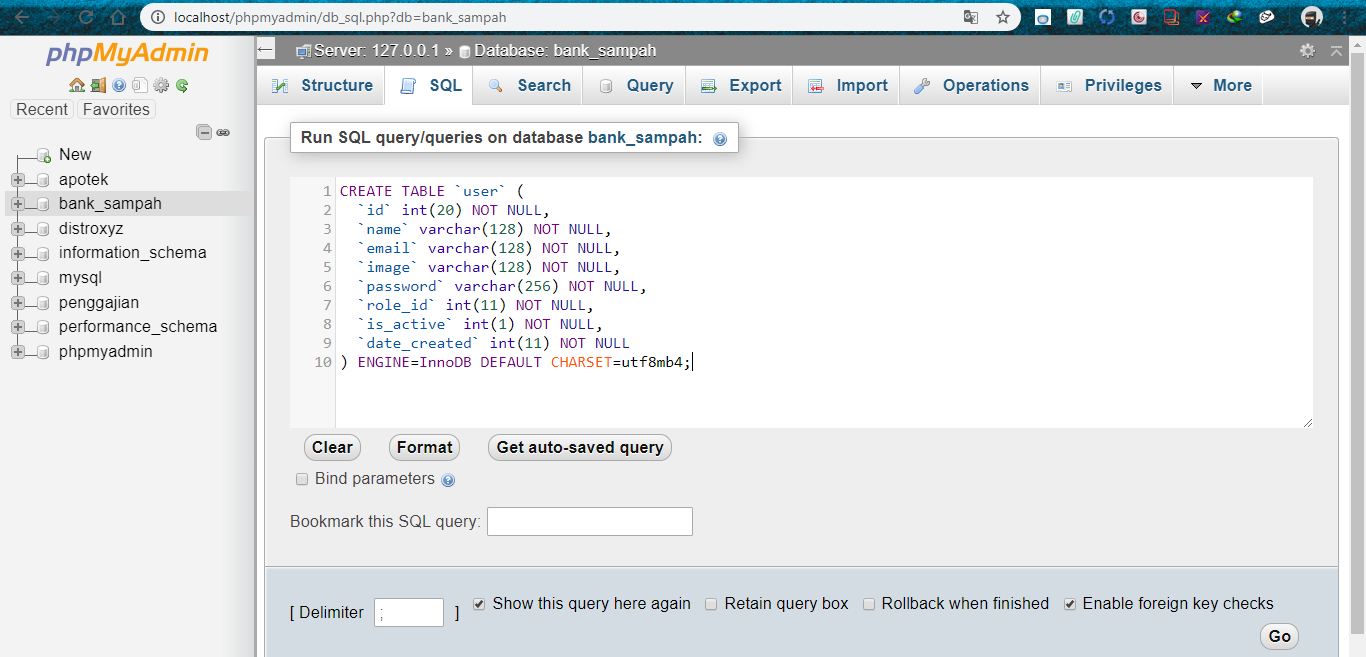
\includegraphics[width=1\textwidth]{figures/database/9.png}
\end{figure}

\noindent
Dilanjut dengan membuat tabel user\_access\_menu. Caranya masih sama dengan sebelumnya, ketikan script berikut dan untuk mengekseskusinya klik Go.

\lstinputlisting[firstline=214, lastline=218, language=SQL]{src/bank-sampah/bank_sampah.sql}

\begin{figure}[H]
\centering
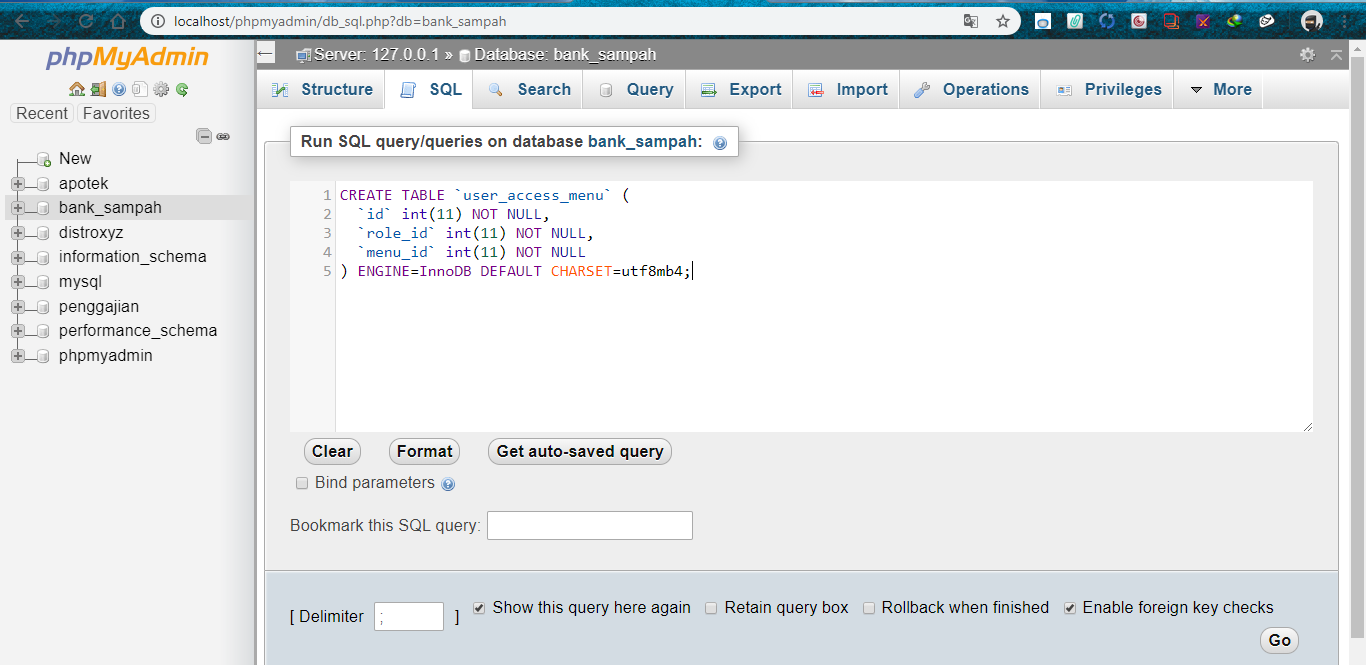
\includegraphics[width=1\textwidth]{figures/database/10.png}
\end{figure}

\noindent
Dilanjut dengan membuat tabel user\_detail. Caranya masih sama dengan sebelumnya, ketikan script berikut dan untuk mengekseskusinya klik Go.

\lstinputlisting[firstline=245, lastline=254, language=SQL]{src/bank-sampah/bank_sampah.sql}

\begin{figure}[H]
\centering
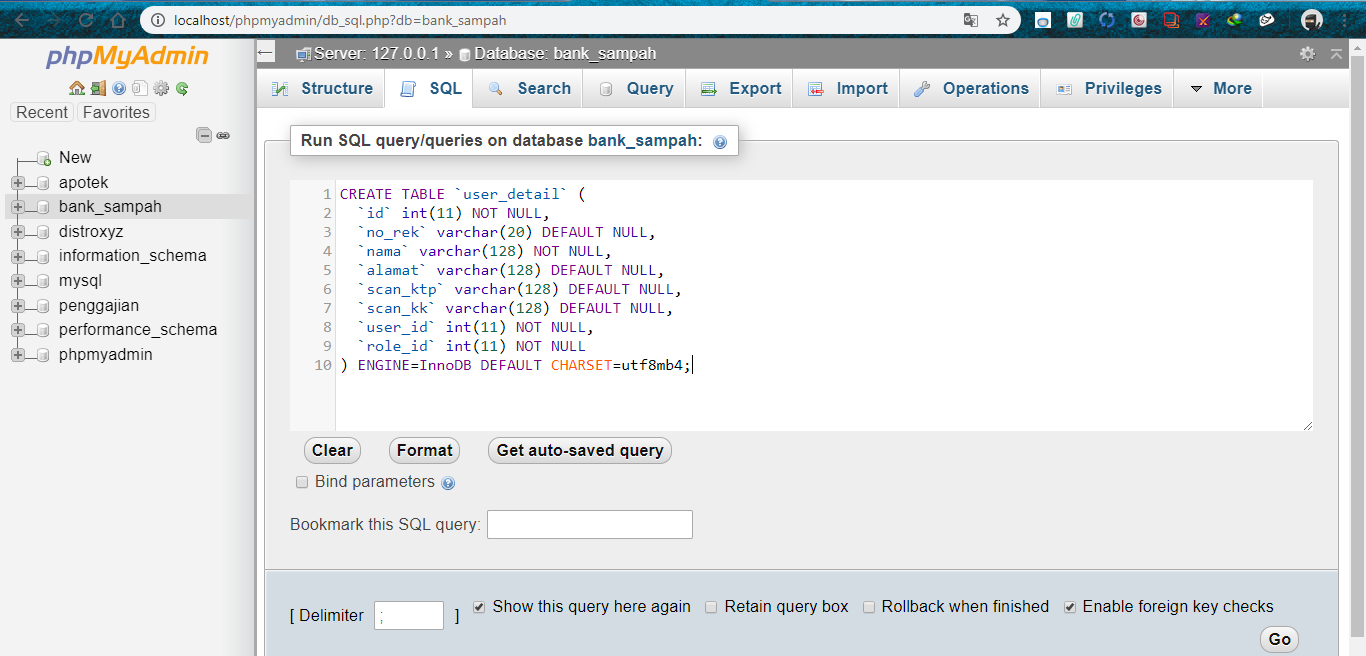
\includegraphics[width=1\textwidth]{figures/database/11.png}
\end{figure}

\noindent
Dilanjut dengan membuat tabel user\_menu. Caranya masih sama dengan sebelumnya, ketikan script berikut dan untuk mengekseskusinya klik Go.

\lstinputlisting[firstline=277, lastline=280, language=SQL]{src/bank-sampah/bank_sampah.sql}

\begin{figure}[H]
\centering
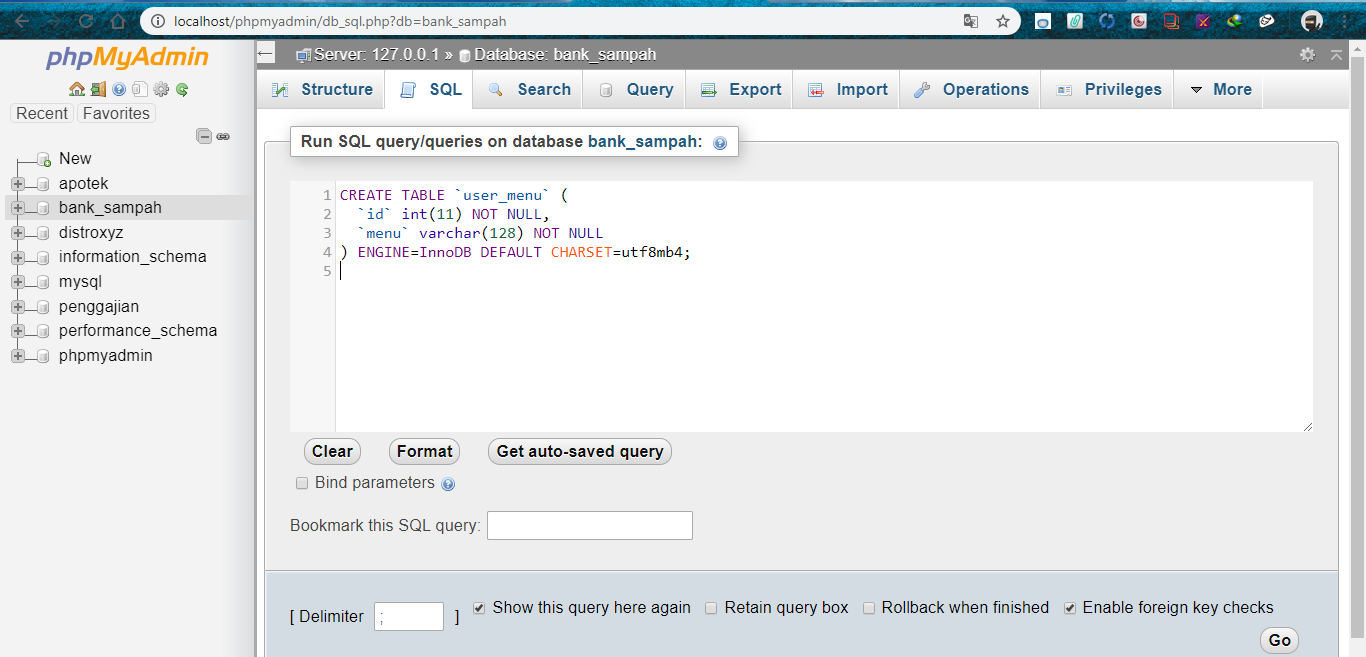
\includegraphics[width=1\textwidth]{figures/database/12.png}
\end{figure}

\noindent
Dilanjut dengan membuat tabel user\_role. Caranya masih sama dengan sebelumnya, ketikan script berikut dan untuk mengekseskusinya klik Go.

\lstinputlisting[firstline=302, lastline=305, language=SQL]{src/bank-sampah/bank_sampah.sql}

\begin{figure}[H]
\centering
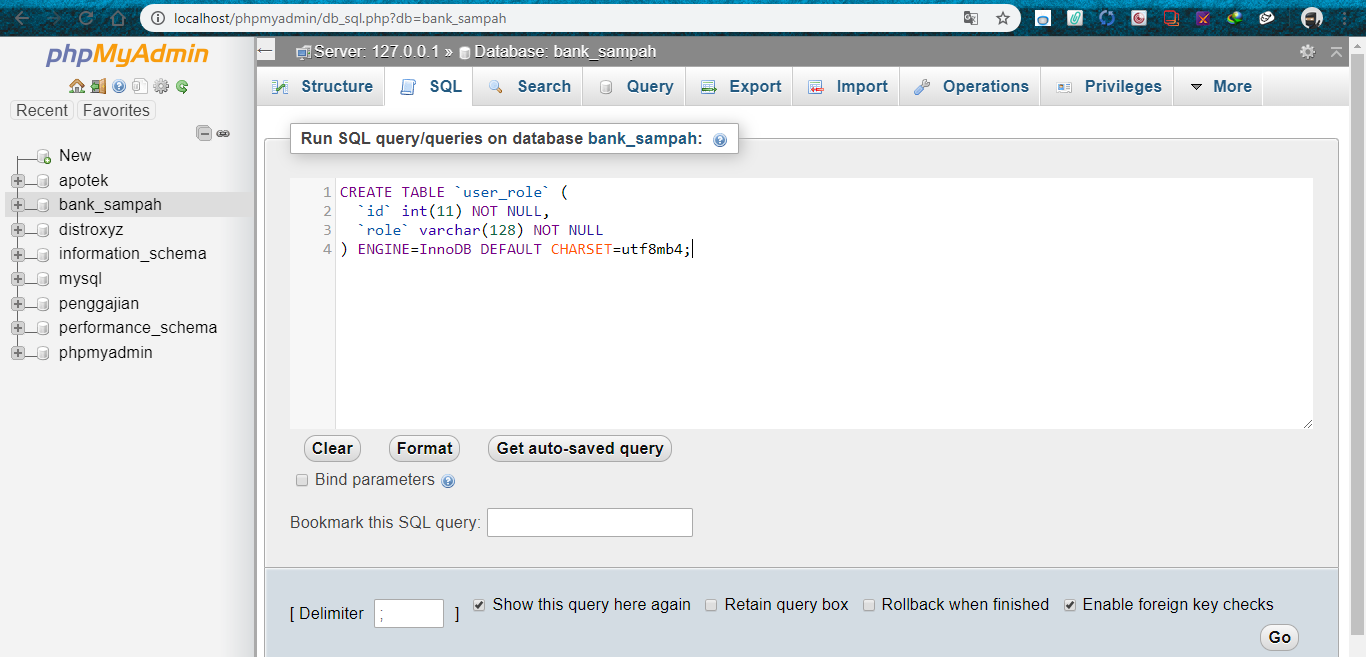
\includegraphics[width=1\textwidth]{figures/database/13.png}
\end{figure}

\noindent
Dilanjut dengan membuat tabel user\_sub\_menu. Caranya masih sama dengan sebelumnya, ketikan script berikut dan untuk mengekseskusinya klik Go.

\lstinputlisting[firstline=323, lastline=329, language=SQL]{src/bank-sampah/bank_sampah.sql}

\begin{figure}[H]
\centering
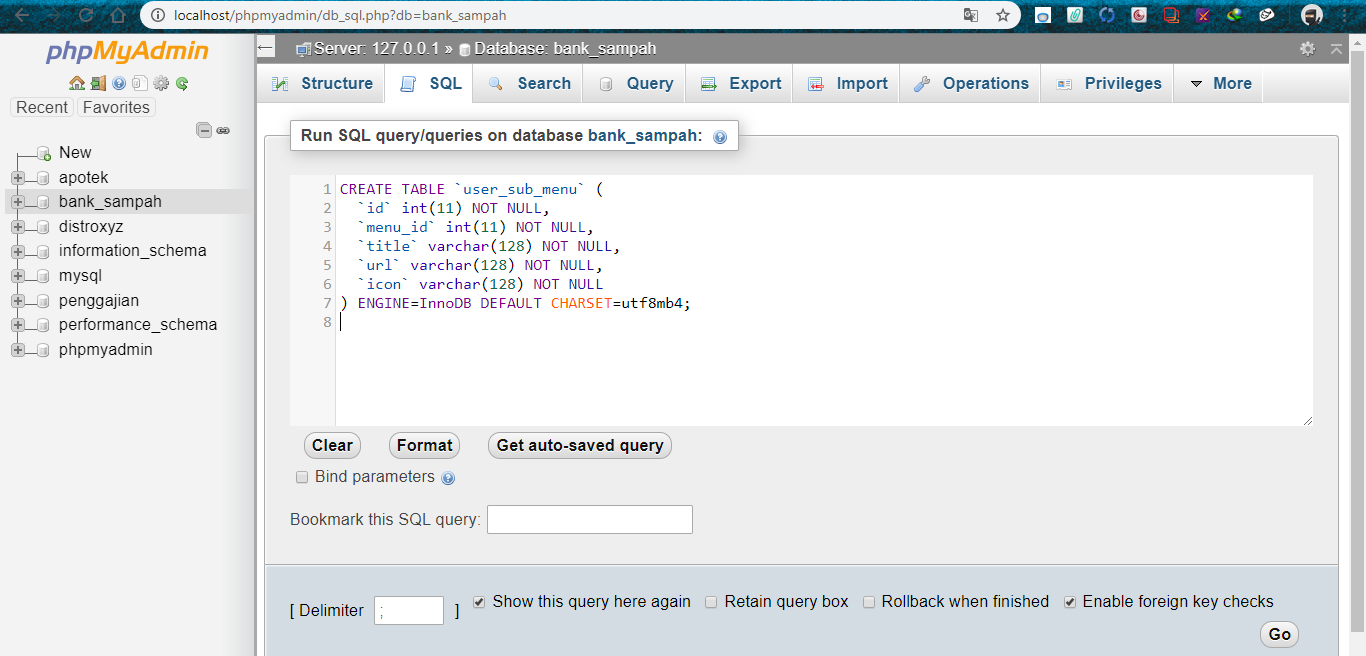
\includegraphics[width=1\textwidth]{figures/database/14.png}
\end{figure}

\noindent
Sehingga hasil akhir dari pembuatan beberapa tabel yang dibutuhkan  tersebut akan seperti ini :

\begin{figure}[H]
\centering
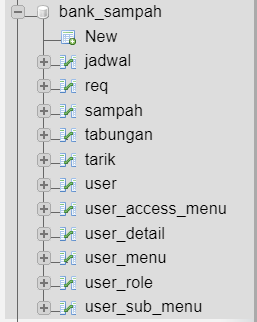
\includegraphics[width=1\textwidth]{figures/database/15.png}
\end{figure}

\begin{figure}[H]
\centering
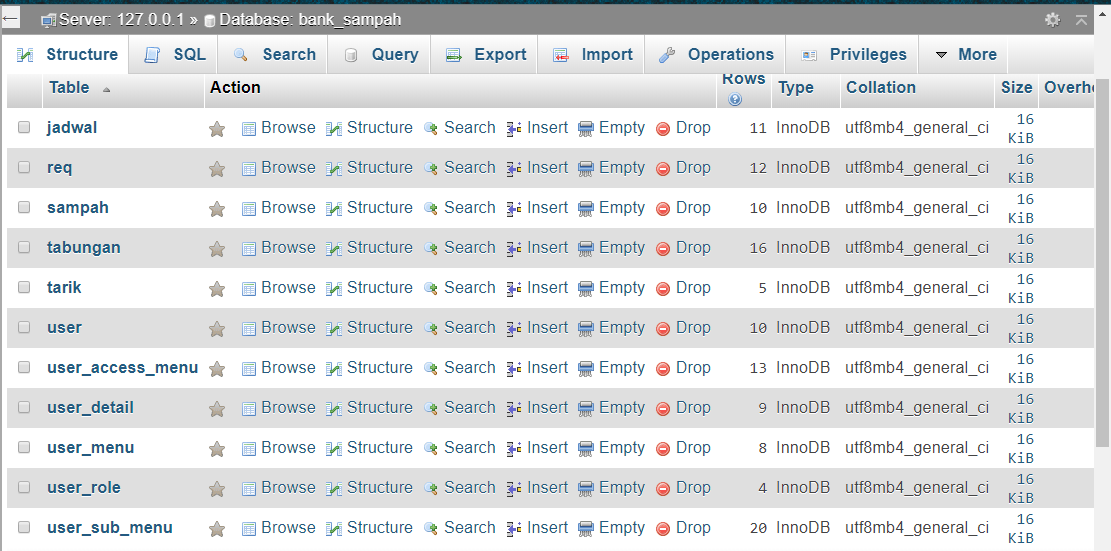
\includegraphics[width=1\textwidth]{figures/database/16.png}
\end{figure}

\noindent
Kurang lebih ada 11 tabel yang berhasil kita buat pada database bank\_sampah.